\documentclass{beamer}

\usepackage{graphicx}
%\usepackage[english]{babel}
\usepackage[utf8x]{inputenc}
\usepackage{anyfontsize}
\usepackage{ragged2e}
\usepackage{subfig}
\usepackage{array}
\usepackage{multirow}
\usepackage{xcolor}
\usepackage{algorithm}
\usepackage{algpseudocode}
\usepackage[orientation=landscape,size=custom,width=16,height=9.75,scale=0.5,debug]{beamerposter}

\renewcommand\footnoterule{}
\definecolor{mmvlabRed}{RGB}{153,0,0}
\usetheme{mmvlab}

\title[]{Fog Computing}
\author{Msc. Daniel Barrag\'an Calde\'on \\ Eng.Augusto G\'omez Vinasco \\
Universidad del Valle}

\begin{document}

\setbeamertemplate{footline}[mmvlab]

\begin{frame}[plain]
  \titlepage
\end{frame}


\begin{frame}{Outline}
\begin{minipage}[t][4cm][t]{\textwidth}
\tableofcontents
\end{minipage}
\end{frame}

\section{General Idea}

\setbeamertemplate{frametitle}[mmvlab]
\setbeamertemplate{footline}[mmvlab]

\begin{frame}{General Idea}
\justifying
Emerging coding technologies beyond HEVC. Specifically \textbf{sparse representation for coding} using fog-computing. The basic idea is to do the \textbf{main analytics} at the source (can be in the cloud), \textbf{encode sparse information} and then do \textbf{distributed up-sampling} at the network edge (close to the sink). This is very appealing in the context of the new MPEG ad-hoc group starting right now
\end{frame}

\section{Problem Statement}

\begin{frame}{Problem Statement}
\begin{itemize}
\item Undergraduate level
\item Master level
\item Ph. D. level
\end{itemize}
\end{frame}

\section{Objectives}

\begin{frame}{Objectives}
Coming soon...
\end{frame}

\setbeamertemplate{frametitle}[diagram]
\setbeamertemplate{footline}[diagram]

\section{Cloud Computing}

\begin{frame}{Cloud Computing}
\centering

\includegraphics[width=0.8\textwidth]{images/cloud}
\foot{source: \url{ http://blog.pyme.pe}}
\end{frame}


\setbeamertemplate{frametitle}[mmvlab]
\setbeamertemplate{footline}[mmvlab]

\begin{frame}{Cloud Computing Concepts}
\begin{itemize}
\item Cloud computing, in fog computing context, refers to high performance hardware, systems software, and applications delivered as services from a third party provider over the Internet
\item Cloud computing has unreliable latency, lacks of mobility support and location-awareness that remains even when the computational power of end-devices is high 
\end{itemize}
\end{frame}

\section{Fog Computing}

\setbeamertemplate{frametitle}[diagram]
\setbeamertemplate{footline}[diagram]

\begin{frame}{Fog Computing Diagram}
\centering
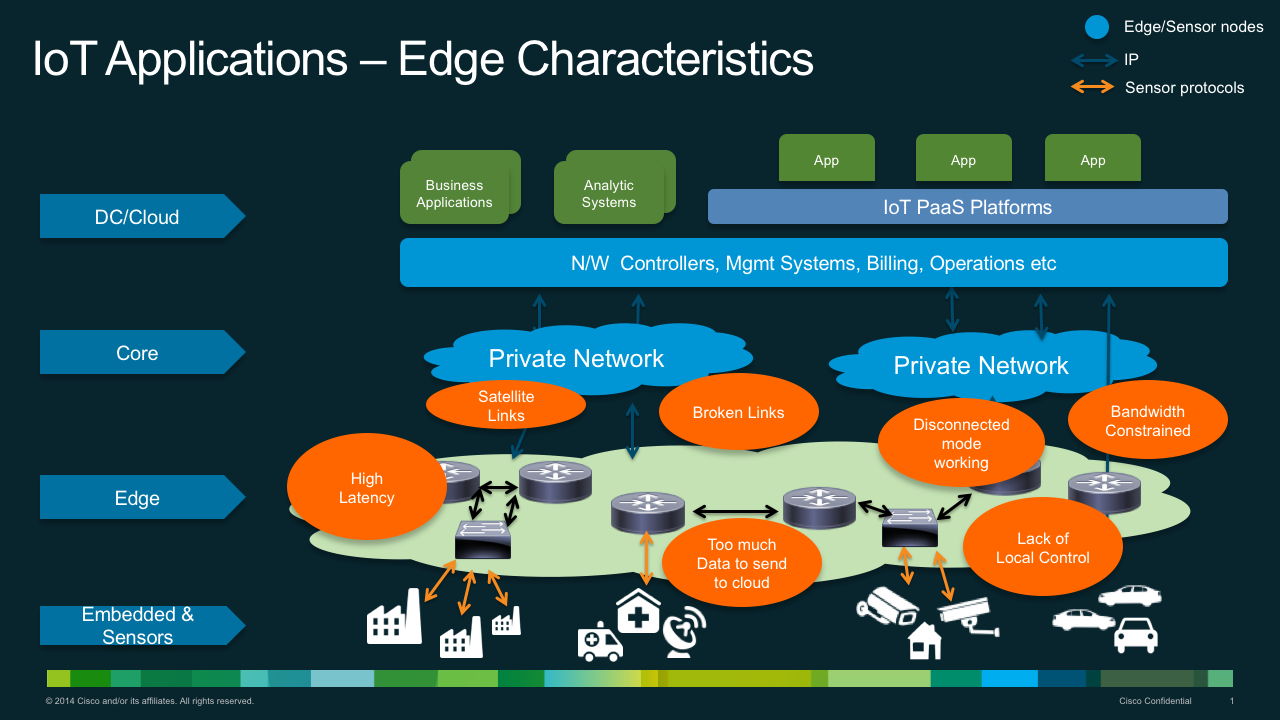
\includegraphics[width=0.8\textwidth]{images/fog}
\foot{source: \url{https://developer.cisco.com/site/iox}}
\end{frame}

\setbeamertemplate{frametitle}[mmvlab]
\setbeamertemplate{footline}[mmvlab]

\begin{frame}{Fog Computing Concepts}
\begin{itemize}
\item Fog computing provide elastic resources and services to end users at the edge of network
\item Fog computing is implement through devices that combine functionalities of data analytics, data storage and networking
\item Fog nodes are devices that can provide resources for services at the edge of the network
\end{itemize}
\end{frame}


\setbeamertemplate{frametitle}[diagram]
\setbeamertemplate{footline}[diagram]

\begin{frame}{Cisco - IOx Framework}
\centering
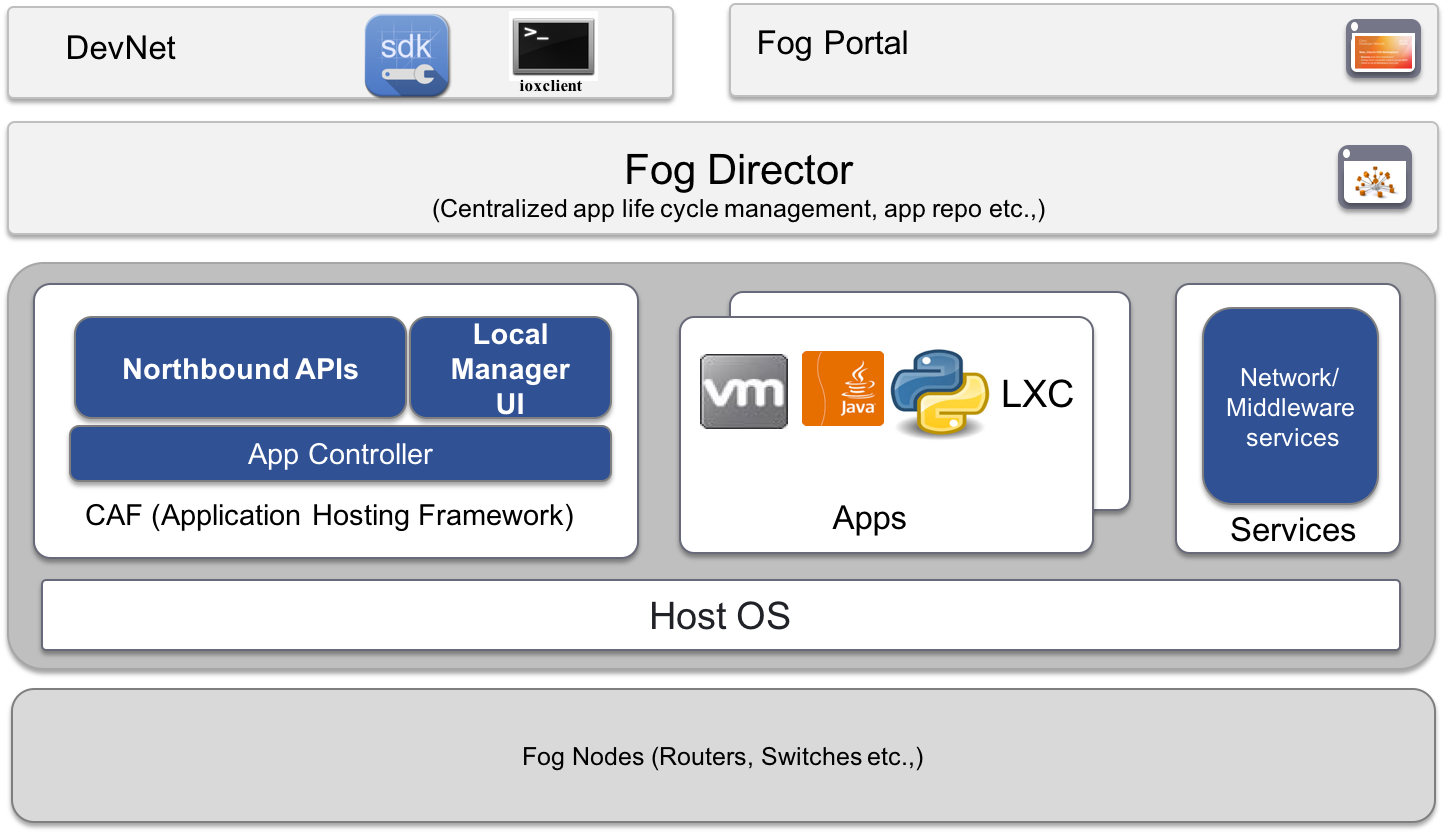
\includegraphics[width=0.8\textwidth]{images/iox}
\foot{source: \url{https://developer.cisco.com/site/iox}}
\end{frame}

\setbeamertemplate{frametitle}[mmvlab]
\setbeamertemplate{footline}[mmvlab]

\begin{frame}{IOx Concepts}
\begin{itemize}
\item IOx is the Cisco framework for devices operating at the network edge to host applications and services along all life cycle (development, distribution, deployment, hosting, monitoring and management)
\item IOx has three application types, they are PaaS Style, VM Style and Container style (application code, 3rd party dependent libraries, native)
\end{itemize}
\end{frame}

\begin{frame}{Cloudlet}
Cloudlet is a trusted, resource-rich computer or cluster of computers that is well connected to Internet and available for use by nearby mobile devices
\end{frame}

\setbeamertemplate{frametitle}[diagram]
\setbeamertemplate{footline}[diagram]

\begin{frame}{Docker Container}
\centering
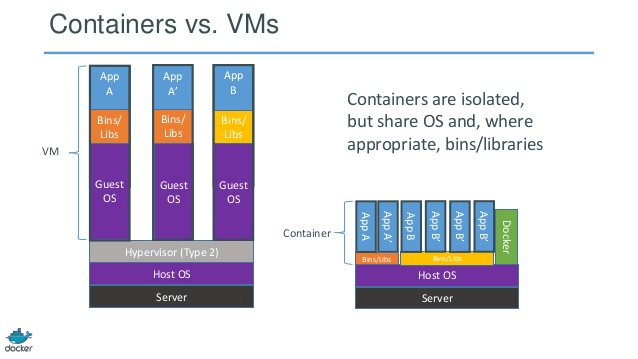
\includegraphics[width=0.8\textwidth]{images/docker}
\foot{source: \url{http://www.zdnet.com}}
\end{frame}

\setbeamertemplate{frametitle}[mmvlab]
\setbeamertemplate{footline}[mmvlab]

\begin{frame}{Container Concepts}
\begin{itemize}
\item Docker is an open platform for developers and sysadmins to build, ship, and run distributed applications, whether on laptops, data center VMs, or the cloud
\item LXC (Linux Containers) is an operating-system-level virtualization method for running multiple isolated Linux systems (containers) on a control host using a single Linux kernel
\end{itemize}
\end{frame}

\setbeamertemplate{frametitle}[diagram]
\setbeamertemplate{footline}[diagram]

\begin{frame}{Software-defined Network (SDN)}
\centering
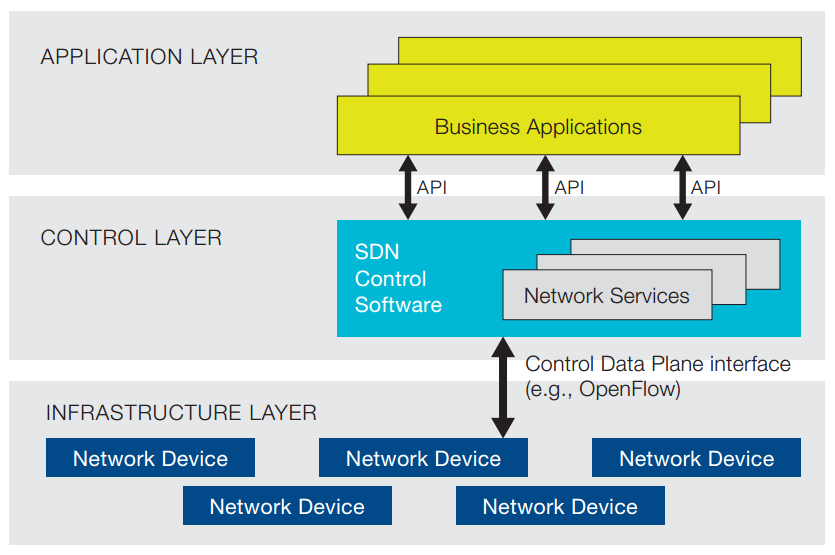
\includegraphics[width=0.7\textwidth]{images/sdn}
\foot{source: Open Networking Foundation - White Paper}
\end{frame}

\setbeamertemplate{frametitle}[mmvlab]
\setbeamertemplate{footline}[mmvlab]

\begin{frame}{SDN Concepts}
Software Defined Networking is an emerging network architecture where network control is decoupled from forwarding and is directly programmable
\end{frame}

\begin{frame}{Content Delivery Network (CDN)}
Content Delivery Network is a globally distributed network of proxy servers deployed in multiple data centers. The goal of a CDN is to serve content to end-users with high availability and high performance
\end{frame}

\setbeamertemplate{frametitle}[diagram]
\setbeamertemplate{footline}[diagram]

\section{MPEG-DASH}

\begin{frame}{MPEG-DASH}
\centering
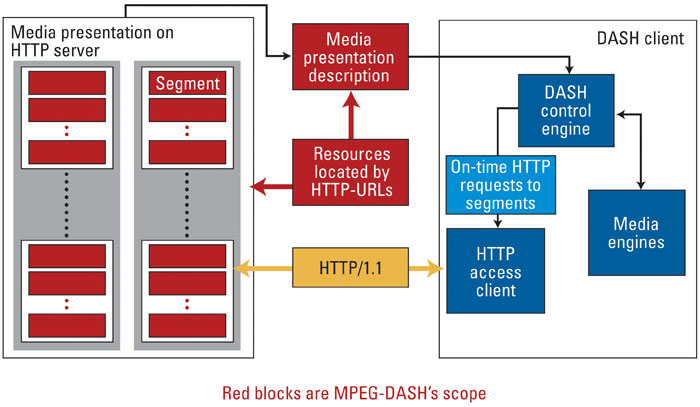
\includegraphics[width=0.7\textwidth]{images/dash}
\foot{source: \url{http://www.tvtechnology.com/cable-satellite-iptv/0149/mobile-video-delivery/235555}}
\end{frame}

\setbeamertemplate{frametitle}[mmvlab]
\setbeamertemplate{footline}[mmvlab]

\begin{frame}{MPEG-DASH Concepts}
MPEG-DASH is an ISO standard for Dynamic Adaptive Streaming over HTTP. Adaptive streaming defines Segments that are a few seconds long and a playlist format that describes alternative encodings of each Segment with different bitrates, resolutions, codecs, etc.
\end{frame}

\begin{frame}{General Concepts}
\begin{itemize}
\item Computation offloading refers to the transfer of certain computing tasks to an external platform, such as a cluster, grid, or a cloud
\item A white paper is an informational document issued by a company to promote or highlight the features of a solution, product or service
\end{itemize}
\end{frame}

\begin{frame}{References}
\vskip0.4cm
\small
\begin{itemize}
\item [1] Shanhe Yi. A Survey of Fog Computing: Concepts, Applications and Issues
\item [2] L. M. Vaquero and L. Rodero-Merino. Finding your way in the fog: Towards a comprehensive definition of fog computing
\item [3] MPEG-DASH: The Standard for Multimedia Streaming Over Internet. White Paper
\item [4] \url{https://developer.cisco.com/site/iox/documents/developer-guide/}
\item [5] \url{https://www.opennetworking.org/about/onf-overview}
\item [6] \url{http://elijah.cs.cmu.edu/}
\item [7] \url{https://www.akamai.com/es/es/}
\item [8] \url{http://www.encoding.com/mpeg-dash/}
\item [9] \url{http://www.bogotobogo.com/VideoStreaming/mpeg_dash.php}
\end{itemize}
\end{frame}

\section{}

\begin{frame}{\Huge{THANKS!!!}}
\vskip0.5cm
\begin{figure}
\centering
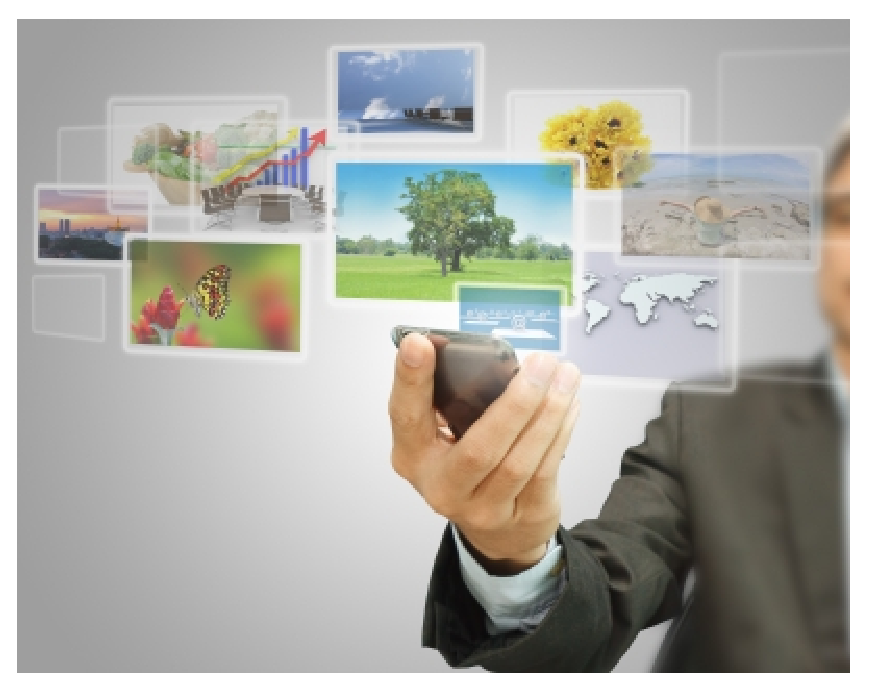
\includegraphics[scale=0.5]{images/image.eps}
\end{figure}
\end{frame}




\end{document}